\documentclass[../main.tex]{subfiles}

\begin{document}
\chapter{Results}
\label{ch:results}

In chapter~\ref{ch:benchmarks} I described the creation of a benchmark
to test the \gls{ir} agent created in chapter~\ref{ch:agent}.
This chapter presents the results.
First, the results for four different chatbot services will be compared
section~\ref{sec:benchmark_results}.
I compare the result of GPT-3-Turbo, GPT-4-Turbo, Perplexity AI and the \gls{ir}
agent.
The small size of the dataset does not allow general statements about
answer quality for the \gls{ir} agent.
Therefore, section~\ref{sec:subjective_evaluation} looks at exemplary question and answer
pairs to compare the answer quality.
While generating the answer for the benchmark, the \gls{ir} agent had some failed runs.
The patterns that lead to failed runs are described in section~\ref{sec:pof}.

While working with \gls{autogpt} and developing the \gls{ir} agent,
a couple of weaknesses of current \gls{llm} agent systems became visible.
The most important challenge for \gls{llm} agents is the non-deterministic generation of large language models.
It makes it significantly harder to build a software system around it because every time the language model is called,
there has to be a fallback mechanism in case something fails.
For fixed pipeline systems this is true as well,
but error handling is easier as the task steps are known beforehand.

\section{Benchmark Results}
\label{sec:benchmark_results}

In chapter~\ref{ch:benchmarks} a benchmark to test the \gls{ir} agent was created.
The benchmark consists of a small \gls{qa} set with eight pairs.
Testing the \gls{ir} agent was done manually using the \gls{autogpt} web interface.
I copied the question in the prompt window without any extra guidance for the agent.

The agent was compared to the free version of Perplexity AI,
GPT-3.5-Turbo and GPT-4-Turbo.
To generate the answers of Perplexity AI, I pasted the question into the prompt window in the
same way as with the \gls{ir} agent.
For the \gls{gpt} models, I used the API functions.

\pgfplotsset{every axis plot/.append style={line width=0.2pt}}
\begin{figure}[ht]
      \centering
      \begin{tikzpicture}
            \begin{axis}[
                        ybar=0pt,
                        ymin=0.3,
                        ymax=1,
                        legend cell align={left},
                        width=\textwidth,
                        height=\textheight/2.5,
                        ylabel={Cosine Similarity},
                        xlabel=Question,
                        bar width=0.25cm,
                        tickwidth=0pt,
                        y axis line style={opacity=0},
                        legend pos=north west,
                        symbolic x coords = {
                                    Q1, Q2, Q3, Q4, Q5, Q6, Q7, Q8, Q9
                              }
                  ]
                  \addplot [
                        draw,
                        fill=blue!30,
                        %postaction={pattern={Lines[angle=45, distance=4pt]}}
                  ] coordinates {
                              (Q1, 0.67)
                              (Q2, 0.40)
                              (Q3, 0.52)
                              (Q4, 0.68)
                              (Q5, 0.80)
                              (Q6, 0.73)
                              (Q7, 0.76)
                              (Q8, 0.58)
                        };
                  \addplot [
                        draw,
                        fill=yellow!30,
                        % postaction={pattern=crosshatch dots}
                  ] coordinates {
                              (Q1, 0.67)
                              (Q2, 0.54)
                              (Q3, 0.53)
                              (Q4, 0.63)
                              (Q5, 0.77)
                              (Q6, 0.76)
                              (Q7, 0.75)
                              (Q8, 0.68)
                        };
                  \addplot [draw, fill=green!30,
                        % pattern={Lines[angle=-45, distance=4pt]}
                  ] coordinates {
                              (Q1, 0.69)
                              (Q2, 0.47)
                              (Q3, 0.54)
                              (Q4, 0.68)
                              (Q5, 0.81)
                              (Q6, 0.78)
                              (Q7, 0.75)
                              (Q8, 0.62)
                        };
                  \addplot [draw, fill=red!30,
                        % pattern=horizontal lines
                  ] coordinates {
                              (Q1, 0.69)
                              (Q2, 0.36)
                              (Q3, 0.61)
                              (Q4, 0.69)
                              (Q5, 0.77)
                              (Q6, 0.70)
                              (Q7, 0.82)
                              (Q8, 0.66)
                        };
                  \legend{GPT-3.5-Turbo, GPT-4-Turbo, Perplexity AI, IR Agent}
            \end{axis}
      \end{tikzpicture}
      \caption{Semantic distances between the gold standard answer and the generated answer.
            The semantic distance is calculated as the cosine distance of the sentence embeddings.}
      \label{fig:benchmark_results}
\end{figure}

The benchmarking results are shown in figure~\ref{fig:benchmark_results}.
We can observe, that all tested services perform similarly for each question.
No service outperforms the others.
Differences in similarity are visible between questions, hinting at some questions being
more difficult to answer than others.
The main reasons for these results are the choice of question-answer pairs, and using the
cosine similarity to measure the answer quality.

The eight questions used in the benchmark are not nearly enough to capture all
kinds of questions possible, and make quantitative statements.
Therefore, the next section will provide a qualitative of the agent answers.

\section{Qualitative Evaluation}
\label{sec:subjective_evaluation}

This section will give a qualitative evaluation of the benchmark results shown
in section~\ref{sec:benchmark_results}.
I will discuss some examples for \gls{qa} pairs that had good results and some
with bad results.
While these examples do not allow for statistically relevant statements about
the agent performance, they can still provide useful insights.

\subsection{Good Example}

The agent was able to generate a good answer for question eight:
\begin{quote}
      Who was likely the user of the portable breviary from San Zeno Maggiore?
\end{quote}
The corresponding answer is:
\begin{quote}
      ``The fact that the breviary transmits texts decidedly pertinent
      to the abbot reveals quite clearly that the book was intended
      for no less than \textcolor{emph blue}{the abbot of San Zeno Maggiore}.''
\end{quote}
The generated answer of the \gls{ir} agent contains the correct statement:
\begin{quote}
      ``The user of the portable breviary from San Zeno Maggiore was likely
      \textcolor{emph blue}{the abbot} for personal use rather than for the monastic
      community's collective ritual practices. <id:1>``
\end{quote}
Here, the retrieval worked better,
and the agent added a document ID after the answer,
indicating it used the first document from the five retrieved documents as context.
Indeed, document one contains the relevant information to answer the question:
\begin{quote}
      ``late-fifteenth-century breviary from the Abbey of San Zeno [\dots]
      it was probably made for the abbot's personal use rather than
      for the monastic community's collective ritual practices.''
\end{quote}
In this case, all agent steps have worked.
First, when adding the article to the database the required information stayed
together in a single chunk.
Then, the agent was able to generate a query to the database that yielded the
relevant chunk.
Finally, the \gls{rag} call to the \gls{llm} produced an answer that relied on that
specific chunk.

\subsection{Bad Example}

The worst answers were produced for short questions that did not contain a lot of context.
All tested services performed worst for question two,
which asks for a term definition:
\begin{quote}
      ``What is a qersu?''
\end{quote}
The article passage used as ground truth is:
\begin{quote}
      ``Some consultations took place in \textcolor{emph blue}{a sacred enclosure}
      by the river \textcolor{emph blue}{called a qersu}.''
\end{quote}
This is a hard example, as the question contains minimal context for the term ``qersu''.
As we will see, the word is used to describe multiple things.

In figure~\ref{fig:benchmark_results} we can see that GPT-4 gave the best answer,
while the \gls{ir} agent produced the worst.
The \gls{ir} agent answer is not a wrong term definition,
but the agent completely fails at answering the question.
The output of the \gls{ir} agent is
\begin{quote}
      ``I'm sorry, but the term 'qersu' is not mentioned in the provided context documents. <?>''
\end{quote}
This would be a good result if the agent did not have access to any sources
containing the necessary information.
In this case, the journal was added to the agent database, so ideally an actual
answer defining the term should be generated.
Answers of this kind hint at problems in the retrieval step.
I will look at retrieval problems in more detail in section~\ref{sec:pof}.

In comparison, the GPT-4 answer includes the sentence:
\begin{quote}
      ``[\dots] In Hittite culture, \textcolor{emph blue}{a ``qersu'' was}
      essentially \textcolor{emph blue}{a type of temple or sanctuary}. [\dots]''
\end{quote}
Remember that GPT-4 was prompted without additional context,
which means that this information was learned during the pre-training phase of GPT-4.

Interestingly, \gls{ppai} answer and provides sources,
but returns a different definition of the term:
\begin{quote}
      ``A ``qersu'' is a type of coffin characterized by [\dots] in Ancient Egypt.''
\end{quote}
It also provides a source that supports the claim but chooses a different one
from the web.
Note that I did not upload the journal as a source for \gls{ppai}, this might
have yielded a better answer.

We have seen that there are different reasons for the bad answer of the \gls{ir} agent.
In the next section, I will put these reasons in several categories.

\section{Points of Failure}
\label{sec:pof}

While testing the \gls{ir} agent, different types of errors occurred.
In this section, I will describe the three main problems I found, ability choice,
complying with the system format, and retrieval errors.

Due to the non-deterministic generation of \glspl{llm},
different answers can be generated for the same prompt.
The answer is likely semantically similar to the previous one,
but when a model has to choose between two abilities,
a small difference can decide if the agent succeeds or fails at completing the task.

Another challenge when developing agents
is the natural language interface of \glspl{llm}.
While it makes describing the task easier for humans,
it complicates the internal communication in the software.
For example,
\gls{autogpt} needs the agent to answer in a structured system format.
While this works most of the time,
it is not guaranteed that the answer complies with the format.
A small deviation such as a missing bracket can break the parsing process.

Retrieval problems can have different reasons but have the same result.
The agent tries to generate an answer using context documents that are
non-relevant to the question.

\subsection{Ability Choice}

\begin{figure}[t]
      \centering
      \begin{tikzpicture}[
                  ab/.style={ability, minimum height=2cm, align=left}]
            \node[minimum height=2cm, align=left] (prompt) {What is\\a 'qersu'?};
            \node[ab, right=of prompt, label={retrieve}] (step1) {Chunk1\\\dots\\Chunk5};
            \node[ab, draw=emph red, right=of step1, label={read\_file}] (step2) {Doc 1: Chunk 1\\\dots\\Doc 5: Chunk 5};
            \node[ab, right=2cm of step2, label={write\_file}] (step3) {VGhlIH\\NlYXJja\\CBmb3I\\\dots};
            \node[right=of step3] (finish) {finish};
            \draw[->] (prompt) -- (step1);
            \draw[->] (step1) -- node[above, align=center] {file} (step2);
            \draw[->] (step2) -- node[above, align=center] {prompt\\context} (step3);
            \draw[->] (step3) -- (finish);
      \end{tikzpicture}
      \caption{An agent run that failed because of an incorrect action choice.
            The agent read the context file into the next prompt,
            instead of using it for the answering ability.
            In the last step, it still produced an output file,
            so for an outside observer that only looks at input and output,
            the agent behaved correctly, but the answer is just random characters.}
      \label{fig:bad_agent_run}
\end{figure}

The agent sometimes chooses abilities that are not suited to progress towards the goal.
For example, when the agent has read and write abilities, the agent decides to
read the file containing the retrieved context in some instances.
The correct choice would have been to proceed with the ``answer'' ability.
In some instances, choosing the wrong ability leads to useless answers,
as shown in figure~\ref{fig:bad_agent_run}.

A solution to this problem is to either remove the read and write abilities
or to guide the agent with explicit instruction in the prompt on which ability to use.
For a true autonomous agent, these solutions are not ideal, because we want the
agent to make the decisions with minimal user intervention.
Fixes like removing abilities bring the agent closer to fixed pipeline solutions.
Another solution could be to retry the same or modified prompts.
This is feasible if the user does not demand fast responses.
In the case of \gls{ir}, the agent should answer reasonably fast and
give correct answers.
Therefore, I opted to remove all abilities that were not needed for \gls{rag}.

Furthermore, the model choice is important for decision-making.
GPT-4 is a lot better than GPT-3 at making good decisions, following tasks, and providing
criticism and reasoning.
For this reason, GPT-4 was used as the agent controller \gls{llm}.

\subsection{LLM Answer Format}

After receiving the answer to the step prompt, the agent has to parse it.
The parsing step can only work if the answer is generated in the exact format specification.
It is not certain that an \gls{llm} adheres to the system format.

Larger models like GPT-4 are better than smaller ones like GPT-3, but also cost more.
Other models improve at structured answers with fine-tuning
but might lose capabilities in other areas as a result.
A software-based solution could be to catch common mistakes from \glspl{llm}
such as missing brackets or missing commas in JSON.
While some mistakes can be mitigated with this approach, it is not feasible
for large-scale applications as there are too many places where the format can break.
Similar to ability choice mistakes, another solution is to retry
and hope for a parsable answer.
I chose this option to develop and test the \gls{ir} agent.

\subsection{Document Retrieval}

There are two main reasons for failed retrieval of context for a user question,
bad chunking and implicit query rewriting.
In section~\ref{sec:subjective_evaluation} we have seen an example question where
the agent could not answer the question given the retrieved context.
This should not happen, as the dataset questions are based on the content the agent has access to.
An answer of this kind hints at problems in the retrieval step before answering.
I identified two main reasons for bad retrieval of information for a question,
bad chunking and implicit query rewriting.

\lstinputlisting[
      style=Code,
      float=tp,
      caption={An example of bad chunking.
                  Additional information splits the article content into two parts.
                  This can hinder the quality of the produced embeddings,
                  as the chunk has semantically mixed content.},
      captionpos=b,
      label={lst:two_page_chunk}]{include/code/two_page_chunk.txt}

Bad chunking happens in the ingestion step, where to source document is added to the
vector database.
The chunking strategy of the \gls{ir} agent is very simple, the full journal text
is split at sentence level, until the resulting splits reach a desired length.
In some instances, this strategy splits articles and paragraphs at places
where the semantics do not change.
In other cases, one chunk contains unrelated sections of a text.
Both types of bad chunking decrease the quality of the embeddings because the
chunk does not have a single, clear ``meaning'',

Implicit query rewriting happens every time the \gls{ir} agent chooses the retrieve ability.
The retrieval ability has a ``query'' parameter that is set when the \gls{llm}
answers to the step prompt.
It is the task of the language model to convert the user prompt into a query
to the vector database.
Which query retrieves the best documents for the following answer generation is not clear.


\end{document}